\documentclass[twocolumn]{aastex62}
\usepackage{amssymb,amsmath,amsopn}
%% The default is a single spaced, 10 point font, single spaced article.
%% There are 5 other style options available via an optional argument. They
%% can be envoked like this:
%%
%% \documentclass[argument]{aastex62}
%% 
%% where the layout options are:
%%
%%  twocolumn   : two text columns, 10 point font, single spaced article.
%%                This is the most compact and represent the final published
%%                derived PDF copy of the accepted manuscript from the publisher
%%  manuscript  : one text column, 12 point font, double spaced article.
%%  preprint    : one text column, 12 point font, single spaced article.  
%%  preprint2   : two text columns, 12 point font, single spaced article.
%%  modern      : a stylish, single text column, 12 point font, article with
%% 		  wider left and right margins. This uses the Daniel
%% 		  Foreman-Mackey and David Hogg design.
%%  RNAAS       : Preferred style for Research Notes which are by design 
%%                lacking an abstract and brief. DO NOT use \begin{abstract}
%%                and \end{abstract} with this style.
%%
%% Note that you can submit to the AAS Journals in any of these 6 styles.
%%
%% There are other optional arguments one can invoke to allow other stylistic
%% actions. The available options are:
%%
%%  astrosymb    : Loads Astrosymb font and define \astrocommands. 
%%  tighten      : Makes baselineskip slightly smaller, only works with 
%%                 the twocolumn substyle.
%%  times        : uses times font instead of the default
%%  linenumbers  : turn on lineno package.
%%  trackchanges : required to see the revision mark up and print its output
%%  longauthor   : Do not use the more compressed footnote style (default) for 
%%                 the author/collaboration/affiliations. Instead print all
%%                 affiliation information after each name. Creates a much
%%                 long author list but may be desirable for short author papers
%%
%% these can be used in any combination, e.g.
%%
%% \documentclass[twocolumn,linenumbers,trackchanges]{aastex62}
%%
%% AASTeX v6.* now includes \hyperref support. While we have built in specific
%% defaults into the classfile you can manually override them with the
%% \hypersetup command. For example,
%%
%%\hypersetup{linkcolor=red,citecolor=green,filecolor=cyan,urlcolor=magenta}
%%
%% will change the color of the internal links to red, the links to the
%% bibliography to green, the file links to cyan, and the external links to
%% magenta. Additional information on \hyperref options can be found here:
%% https://www.tug.org/applications/hyperref/manual.html#x1-40003
%%
%% If you want to create your own macros, you can do so
%% using \newcommand. Your macros should appear before
%% the \begin{document} command.
%%
\newcommand{\vdag}{(v)^\dagger}
\newcommand\aastex{AAS\TeX}
\newcommand\latex{La\TeX}
\newcommand{\unit}[1]{\ensuremath{\, \mathrm{#1}}}
\newcommand{\figref}[1]{Figure \ref{#1}}

\newcommand{\code}[1]{\ensuremath{\textsf{#1}}}
\newcommand{\lare}{\code{LARE}}
\newcommand{\scipy}{\code{scipy}}
\newcommand{\fnc}[1]{\code{#1}}
\newcommand{\removecomment}[1]{\textcolor{red}{#1}}
\newcommand{\secref}[1]{$\S$\ref{#1}}

% IBIS fitting macros
\newcommand{\halpha}{\ensuremath{H\alpha}}
\newcommand{\hfit}{\ensuremath{\halpha_\mathit{fit} }}
\newcommand{\linecenter}{\ensuremath{\lambda_0}}
\newcommand{\linew}{\ensuremath{\delta \lambda}}
\newcommand{\imin}{\ensuremath{I_\mathit{min}}}
\newcommand{\ihalf}{\ensuremath{I_\mathit{half}}}

% comments
\newcommand{\latcomment}[1]{\textcolor{red}{LAT: #1}}
\newcommand{\saj}[1]{\textcolor{cyan}{SAJ: #1}}
\newcommand{\ark}[1]{\textcolor{purple}{ARK: #1}}

%% Tells LaTeX to search for image files in the 
%% current directory as well as in the figures/ folder.
\graphicspath{{./}{figures/}}

%% Reintroduced the \received and \accepted commands from AASTeX v5.2
\received{January 1, 2022}
\revised{January 7, 2022}
\accepted{\today}
%% Command to document which AAS Journal the manuscript was submitted to.
%% Adds "Submitted to " the arguement.
\submitjournal{ApJ}

%% Mark up commands to limit the number of authors on the front page.
%% Note that in AASTeX v6.2 a \collaboration call (see below) counts as
%% an author in this case.
%
%\AuthorCollaborationLimit=3
%
%% Will only show Schwarz, Muench and "the AAS Journals Data Scientist 
%% collaboration" on the front page of this example manuscript.
%%
%% Note that all of the author will be shown in the published article.
%% This feature is meant to be used prior to acceptance to make the
%% front end of a long author article more manageable. Please do not use
%% this functionality for manuscripts with less than 20 authors. Conversely,
%% please do use this when the number of authors exceeds 40.
%%
%% Use \allauthors at the manuscript end to show the full author list.
%% This command should only be used with \AuthorCollaborationLimit is used.

%% The following command can be used to set the latex table counters.  It
%% is needed in this document because it uses a mix of latex tabular and
%% AASTeX deluxetables.  In general it should not be needed.
%\setcounter{table}{1}

%%%%%%%%%%%%%%%%%%%%%%%%%%%%%%%%%%%%%%%%%%%%%%%%%%%%%%%%%%%%%%%%%%%%%%%%%%%%%%%%
%%
%% The following section outlines numerous optional output that
%% can be displayed in the front matter or as running meta-data.
%%
%% If you wish, you may supply running head information, although
%% this information may be modified by the editorial offices.
\shorttitle{The K\"{o}lsch of Data Sets}
\shortauthors{Kobelski et al.}
%%
%% You can add a light gray and diagonal water-mark to the first page 
%% with this command:
% \watermark{text}
%% where "text", e.g. DRAFT, is the text to appear.  If the text is 
%% long you can control the water-mark size with:
%  \setwatermarkfontsize{dimension}
%% where dimension is any recognized LaTeX dimension, e.g. pt, in, etc.
%%
%%%%%%%%%%%%%%%%%%%%%%%%%%%%%%%%%%%%%%%%%%%%%%%%%%%%%%%%%%%%%%%%%%%%%%%%%%%%%%%%

%% This is the end of the preamble.  Indicate the beginning of the
%% manuscript itself with \begin{document}.

\begin{document}

\title{A publicly available multi-observatory data set of an enhanced network patch from the Photosphere to Corona}
\correspondingauthor{Adam R. Kobelski}
\email{adam.kobelski@nasa.wvu.edu}

\author[0000-0002-4691-1729]{Adam R. Kobelski}
\affiliation{NASA Marshall Space Flight Center}
\affiliation{West Virginia University}


\author[0000-0002-8259-8303]{Lucas A. Tarr}
\affiliation{National Solar Observatory}
%\email{ltarr@nso.edu}
\author[0000-0001-5459-2628]{Sarah A. Jaeggli}
\affiliation{National Solar Observatory}
%\email{sjaeggli@nso.edu}
\author{Nicholas Luber}
\affiliation{West Virginia University}
%% The \author command can take an optional ORCID.
\author[0000-0001-6102-6851]{Harry P. Warren}
\affiliation{Naval Research Laboratory}
%\email{harry.warren@nrl.navy.mil}
\author[0000-0002-6172-0517]{Sabrina Savage}
\affiliation{NASA Marshall Space Flight Center}
%\email{sabrina.savage@nasa.gov}

\begin{abstract}
%Transient brightenings (TBs) are ubiquitous features of the solar atmosphere across many length and energy scales, the most energetic of which manifest as large-class solar flares. TBs typically originate in regions of enhanced magnetic flux and are observed as increased emission across wavelengths from X-ray to radio, with notable dynamics on timescales of seconds to hours. Coronal TBs are often studied using Extreme Ultravioliet (EUV) and X-ray imaging and spectra. TBs likely originate from photospheric activity such as flux emergence, but are proximately driven by energy transfer through the chromosphere, either by convective waves, direct ejection of chromospheric material, or reconnection. Chromospheric and transition region observations of these events have only become routine in the last decade. 
%Chromospheric and transition region observations of these events have not been routine for the last few decades. 
New instruments sensitive to chromospheric radiation at X-ray, UV, Visible, IR, and sub-mm wavelengths have become available that significantly enhance our ability to understand the bi-directional flow of energy through the chromosphere.
We describe the calibration, coalignment, initial results, and public release of a new data set combining a large number of these instruments to obtain multi-wavelength photospheric, chromospheric, and coronal observations capable of improving our understanding of the connectivity between the photosphere and the corona via transient brightenings and wave signatures.
The observations center on a bipolar region of enhanced network magnetic flux near disk center on SOL2017-03-17T14:00-17:00.
The comprehensive data set provides one of the most complete views of chromospheric activity related to small scale brightenings in the corona and chromosphere to date.
Our initial analysis shows strong spatial correspondence between the areas of broadest width of the Hydrogen$\alpha$ spectral line and the hottest temperatures observed in ALMA Band 3 radio data.
The correspondence persists for the duration of cotemporal obserations ($\approx 60\unit{m}$).
Numerous transient brightenings were observed in multiple data series.
We highlight a single well observed transient brightening along a set of thin filamentary features with a duration of 20 minutes.
The timing of the peak intensity transitions from the cooler (ALMA, 7000K) to hotter (XRT, 3MK) data series.
\end{abstract}
\keywords{The Sun, Radio, X-Ray, EUV}

\section{Introduction} \label{sec:intro}
The methods of transporting energy from the photosphere through the chromosphere to the million degree corona have been debated since the discovery of the hot corona \citep[][]{1933LyotMarshall, 1939Grotrian}. 
The underlying problem is that thermal conduction, which is very efficient in solar plasmas, will transport energy from the hot corona to the cool chromosphere from which it rapidly radiates away, so the energy in the corona must constantly be resupplied.
One of the early ideas for this transport of energy was via wave activity through hydrodynamic shocks \citep[][]{1949Schatzman} and later, once the central role of magnetic fields on the Sun was fully realized, by magnetoacoustic or Alfv\'en waves \citep{1961Osterbrock}. 
In this scenario, convective energy drives the waves which carry energy as they propagate upward through to the corona, and eventually deposit that energy as they cascade to small length-scales and heat the plasma through dissipation \citep{2014vanBallegooijenEA_FootpointMotion}.

Coronal waves have been observed in many forms. 
Large amplitude standing and propagating waves are caused by both confined flares and CMEs, and their properties are comparatively easy to detect and quantify \citep{2014LiuOfman_EUVwaves}. 
At the same time, many quiescent coronal structures exhibit continuous oscillatory power, detectable using Fourier transform or wavelet methods of longer time series \citep{Tomczyk:2009}, indicating that a broad spectrum of waves are present throughout the chromosphere and corona.
While the presence of waves is uncontested, where, by what mechanism, and how much wave energy may be dissipated to heat the coronal plasma is currently not well understood \citep{2014vanBallegooijenEA_FootpointMotion}.

As an alternative to wave heating, it has been posited that small-scale magnetic reconnection via nanoflares \citep[][]{1983Parker} could be responsible for the heating of the corona. 
It was thought that these nanoflares would manifest themselves as small scale brightenings in the corona, sometimes referred to as microflares or active region transient brightenings \citep[][]{1984LinEA_microflares, 1991Hudson, 1992ShimizuEA, 1995Shimizu}. 
\citet{1997GaryEA} determined that the small scale-brightenings exhibit the same signatures of particle acceleration as larger solar flares and concluded that many of the transient brightenings (TBs) were also products of magnetic reconnection. 
The details of this connection could have important ramifications for some coronal heating theories,nand is thust still under active study (as seen by the work of Hannah et al, NuStar and MAGIXs, FOXSI among others).
A key suggestion of the Parker nanoflare model was that the reconnection would occur due to substructure in the magnetic field lines, in which the observed loops consist of many unresolved braided magnetic strands. 
The concept of unresolved strands is in agreement with forward models of the observations \citep[e.g.][]{2012BrooksEA, 2014KobelskiEA_XRTTBs, 2014KobelskiMcKenzie_HiC}, and has been strongly suggested by direct observation in extreme ultraviolet (EUV) with the Hi-C sounding rocket \citep[][]{2013CirtainEA_HiC}. 

Microflare research has largely focused on observable transients, which implies ``low-frequency'' active region heating wherein a larger plasma element, such as an overlying coronal loop, is heated significantly enough to show enhanced emission compared to the background and then notably cools over time \citep[][]{2015Klimchuk_CHoverview}. 
This scenario is in contrast to ``high-frequency'' heating wherein the observable plasma elements experience heating events fast enough that they appear at a sustained temperature and density, i.e. they are not allowed to cool or drain between successive heating events. 
Sometimes assumed in this latter paradigm is that the individual microflares occur on unresolved spatial and temporal scales, such that while individual strands may cool and/or drain, the conglomerated strand appears to have a steady average density and temperature \citep[e.g.][]{2013BrooksEA_LoopSize, 2014SubramanianEA_LowAndHighFrequency, 2016SchmelzEA}. 

One of the best ways to follow how plasma flows through the chromosphere and corona is by using emission and absorption spectral measurements. 
For stable loops, raster scans from the \textit{Hinode} EUV Imaging Spectrograph (EIS) and the Interface Region Imaging Spectrograph (IRIS) have been used to better constrain the rate of heating quiescent regions of the Sun \citep[e.g.][]{2016BrooksWarren_NTWidths,2016TestaEA_ARLoopsIRISEIS, 2017GhoshEA_LoopsIRISEIS}. 
To measure flows during transient events requires fortuitous pointing and specific observations with minimal rastering. 
Here we present an ideal data set to study dynamic spectra of small scale, short lived coronal brightenings with coronal, chromospheric, and photospheric instrumentation. 
Such studies are crucial to understanding the flow of energy into the corona, as well as provide statistical insight into this coupled system during solar flares.

Much of the aforementioned work on TBs has focused on the \emph{coronal} observables, though recent instrumentation has shown evidence of chromospheric counterparts to microflaring \citep[][]{2016TestaEA_ARLoopsIRISEIS, 2017GhoshEA_LoopsIRISEIS}. 
The chromospheric response to large flares is well established in the form of chromospheric ablation from flare ribbons \citep[][]{2017Benz_LRSP}. 
The wave-driven chromospheric response to large flares has also been detected and investigated \citep[][and references within]{2014LiuOfman_EUVwaves, 2016RussellEA_Sunquakes}. 
What has eluded prior studies is a comprehensive insight into how wave motion through the chromosphere relates to the occurrence of small coronal flares, as well as how small flares drive chromospheric heating and waves. 
Evidence for this process is given by the partial temporal and spatial overlap of Ellerman bomb populations and UV burst populations, thought to be caused by energetic release at different heights \citep{2019Vissers, 2018Young}.
This feedback loop between waves and transients can inform the bi-directional flow of energy between the chromosphere and the corona.

In this paper, we present a unique, robust, and extensive data set with which to study the flow of energy through the chromosphere and the interplay between transients and wave activity.
Calibrated and coaligned data in FITS format with WCS compliant coordinates are available through a publicly accessible archive hosted at the National Solar Observatory \url{https://share.nso.edu/shared/dkist/ltarr/kolsch/}.
Even though the data set is of a quiescent solar region, it displays notable dynamics from the photosphere to the corona. 
This region is exemplary of the ubiquitous features found throughout the solar atmosphere during all phases of the solar cycle. 
The type of analysis we propose has been performed for active regions and strong plage, \emph{but not quiescent regions}. 
Since this data set probes each layer of the Sun in multiple wavelengths, heights, and temperatures, it can be studied with distinct methodologies, and can provide multiple ground-truths and perspectives for which to compare to models of chromospheric energy flow and transfer in later papers.

The data set includes photospheric magnetic field information from the Helioseismic and Magnetic Imager \citep[HMI,][]{2012SchouEA_HMI} as well as imaging from the Atmospheric Imaging Assembly \citep[AIA,][]{2012LemenEA_AIA} on board the Solar Dynamics Observatory \citep[SDO,][]{2012PesnellEA_SDO}; photospheric magnetic field data from the Solar Optical Telescope \citep[SOT,][]{2008TsunetaEA_SOT}, coronal X-ray imaging from the X-Ray Telescope \citep[XRT,][]{2007GolubEA_XRT}, and EUV spectra from EIS \citep{2007CulhaneEA_EIS} on board the {\it Hinode} spacecraft \citep[][]{2007KosugiEA_Hinode}; chromospheric images and spectra from IRIS \citep{2014DePontieuEA_IRIS}; spectral images from the  Interferometric BIdimensional Spectropolarimeter \citep[IBIS,][]{2006Cavallini_IBIS} and infrared spectropolarimetry from the Facility InfraRed Spectropolarimeter \citep[FIRS,][]{2010JaeggliEA_FIRS} at the Dunn Solar Telescope (DST); and millimeter wave information from the Atacama Large Millimeter Array \citep[ALMA,][]{2009WootenThompson_ALMA, 2010HillsEA_ALMA2}.  For consistency, we refer each individual instrument's collected data as a \emph{data series} and the full collection of data series as the data set.

In this paper, we describe the reduction of the imaging and spectral observations, as well as the co-alignment between instruments. 
We then compare activity between atmospheric layers and provide a preliminary interpretation. 
More thorough analyses are forthcoming. 
We give details of the observations in Section~\ref{sec:data}, their co-alignment in Section~\ref{sec:coalign}, some preliminary analysis in Section~\ref{sec:analysis}, and concluding remarks in \ref{sec:conclusion}. 

\section{Data} \label{sec:data}
\subsection{Overview and Coordination}
\begin{figure}
    \centering
    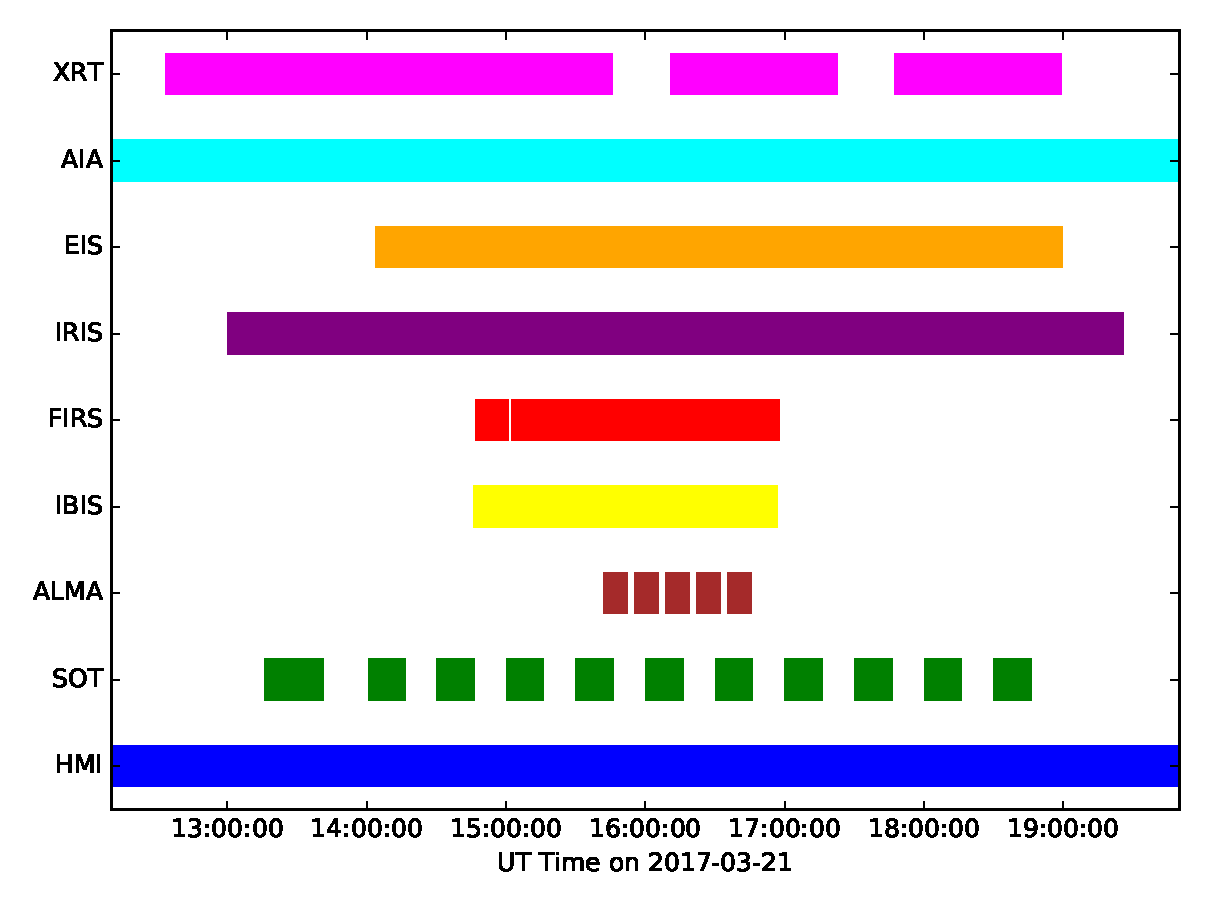
\includegraphics[width=0.95\linewidth]{figures/obs_timing}
    \includegraphics[width=0.48\linewidth]{figures/AIA193_FOVs.png}
    \includegraphics[width=0.48\linewidth]{figures/AIA193_FOVs_zoom.png}
    \caption{Overview of all observations around the ALMA observing window.  Upper plot: timing information, where instruments are ordered vertically roughly according to height in the solar atmosphere.  Gaps in each color band indicate data gaps in that data channel.  Lower panels: approximate FOVs for each instrument using the same colors as in the upper panel, overlaid on an SDO/AIA-193\AA{} context image.}
    \label{fig:coordination}
\end{figure}
The data series presented in this work resulted from a large coordination campaign that was keyed to the ALMA observations and encompassed a suite of ground- and space-based facilities operated by different organizations.
The observations occurred during one of the first coordinated campaigns to support PI-led solar ALMA observations. Due to constraints in the ALMA scheduling, the exact timings and pointings could only be determined the day before the actual observations, with the result that there is not always complete temporal or spatial overlap between each facility.  
Given these constraints, the coverage is, in general, fairly good.

Figure \ref{fig:coordination} presents an overview the temporal and spatial overlap between the various instrument channels during the time of the ALMA observations. 
In the upper panel we have ordered the instruments in the vertical direction roughly according to height in the solar atmosphere.
In addition to the times shown here, SOT, EIS, and XRT took observations of this same region for several days leading up to the ALMA observing window, while SDO and AIA provide near-continuous observations in a variety of wavelengths, as always.
The lower left panels show the approximate fields-of-view (FOV) of the various instruments overlaid on an AIA 193\AA{} image using the same colors as the upper panel, with the left showing the full Sun and the right a zoomed in region.

Figure \ref{fig:coordination2} shows a representative sample of coaligned images from each of the data channels and provides an overview of the target region on the Sun.
The images are approximately co-temporal at 16:27UT and are taken partway though a transient brightening event.
From left to right and top to bottom (and roughly moving from the photosphere through the chromosphere and into the corona) the panels show: 
\begin{itemize}
    {\item (SOT) The photospheric magnetic field including a bipolar region of enhanced network flux}
    {\item (SOT) The solar granulation pattern, including some minor disruptions by the enhanced network concentrations}
    {\item (ALMA) Plasma temperature variations, with hotter/brighter areas roughly coincident with the photospheric magnetic field concentrations}
    {\item (IBIS) \halpha{} blue wing, which shows some dynamic spicules (dark) and the magnetic concentrations (bright)}
    {\item (IBIS) \halpha{} line center, which shows a central sigmoidal filament above the magnetic polarity inversion line}
    {\item (IRIS) Si IV intensity, which shows transient brightenings throughout the FOV, yet mostly concentrated above the enhanced network flux}
    {\item (AIA) 304\AA{} emission, which shows multiple loop brightenings against background of structured emission}
    {\item (AIA) 193\AA{} emission showing multiple loop brightenings}
    {\item (XRT) X-ray emission showing multiple transient strands}
\end{itemize}
We discuss this event in more detail in Section~\ref{sec:analysis} below.
NuSTAR also observed this region and detected two small flares around 19:00 and 19:30 UT \citep{2018Kuhar}, confirming continued X-ray activity after the end of our primary coordinated observations, although we do not condsider the NuSTAR observations in the current study.
The remaining subsections describe each data series from the coordinated observations.
\begin{figure}
    \centering
    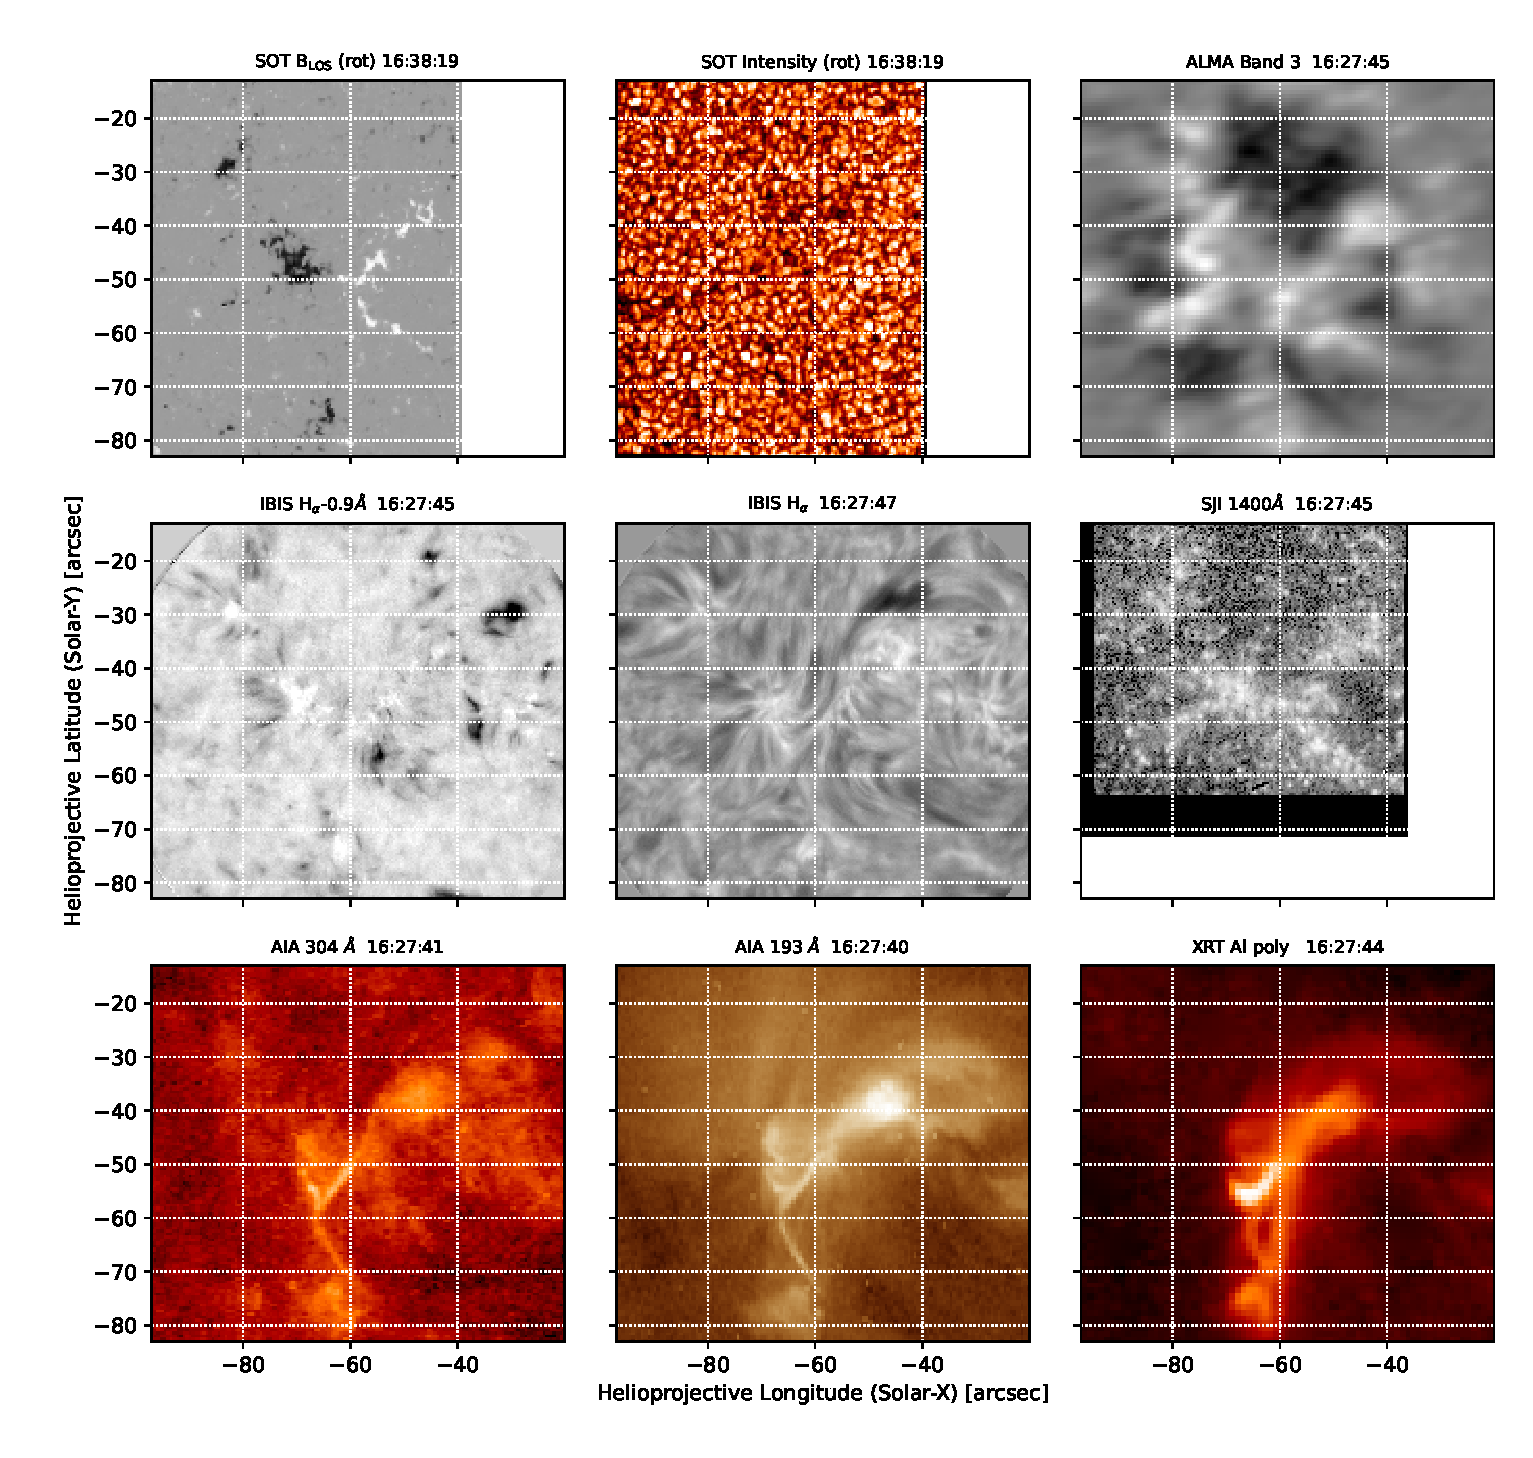
\includegraphics[width=0.95\linewidth]{figures/IBISimg0108.eps}
    \caption{Representative sample of co-aligned images. The SOT data has been rotated to align with the coordinate time of the IBIS data. The ALMA data ranges from $\pm$some number of K}
    \label{fig:coordination2}
\end{figure}

\subsection{SDO/AIA}\label{sec:sdoaia}
AIA obtains full-disk images of the Sun every 12 seconds with 0.6\arcsec{} spatial sampling in a variety of visible, UV, EUV channels.
Observations from all AIA channels are available throughout the entire coordination period.
The Level 1 AIA data was downloaded from the Joint Science Operations Center (JSOC)\footnote{\url{http://jsoc.stanford.edu/}}, updated to Level 1.5 using \fnc{aia\_prep.pro} as described in the SDO Analysis Guide.
We also selected a subregion that fully encompassed the ALMA target using the SSW cutout service\footnote{\url{https://www.lmsal.com/get_aia_data/}; see also \S4.3 of the SDO Analysis Guide.} for a region approximately $300\arcsec\times300\arcsec$ for the duration of the other data series (14:00-17:00 UT on 2017-03-21).
The 193 \AA\ channel of AIA was primarily used for co-alignment and to provide full-disk context for the other observations.  
The 193 \AA\ bandpass includes \ion{Fe}{12} and \ion{Fe}{24} lines which form in the corona and hot plasma at log(T)=6.2 and 7.3 respectively, as described in \citet{2012Boerner} and \citet{2014Boerner}.


\subsection{SDO/HMI}
We used three days of intensity and line-of-site (LOS) magnetograms from the level 1.5 \texttt{hmi.M\_720s} and \texttt{hmi.Ic\_720s} series\footnote{JSOC query: \texttt{hmi.M\_720s[2017.03.19\_00:00:00\_TAI/3d]}, and similar for intensity.}.  
An area $\approx330\arcsec{}\times250\arcsec{}$ was tracked using solar rotation to understand the magnetic evolution of the region leading up to and throughout the coordinated observations.  
To ease later analysis, we derotated all HMI data so that the solar North-South axis aligned with columns of the data array, with North pointing upward, but kept the spatial scaling of the original HMI data.  
The typical extra step of spatially-rescaling the data to match AIA  has little benefit in the present context given that our various data series include many different spatial samplings.

\subsection{ALMA}
\paragraph{ALMA background} The Atacama Large Millimeter Array (ALMA) is a radio interferometer with current frequency coverage spanning 84 to 950 GHz \citep{2009WootenThompson_ALMA}. 
ALMA is constituted of 66 telescope dishes: 54 with a diameter of 12 meters, and 12 with a diameter of 7 meters. 
These 66 dishes are arranged to ensure that ALMA has suitable sensitivity to large-scale diffuse emission, achieved by the high density of centrally located dishes, and excellent resolution to small scale features, achieved with the dishes at long distance. 
For this particular observation, ALMA was in its most compact configuration (C43-1), which limits the small scale resolution, but provides the best available resolution on larger scales, and also minimizes issues caused by water vapor in the Earth's atmosphere above the telescope.
The ALMA observations presented in this work were in the ALMA observing Band 3, which corresponds to a central frequency of 100 GHz, and a total bandwidth of 18 GHz about that central frequency. 
At this frequency and array configuration, our approximate resolution is 2$\arcsec$ on the sky. 
Our integration time is 2 seconds, and the entire observation, including the target field and calibrators, had a duration of 1.03 hours. 

\paragraph{ALMA calibration} The ALMA Band 3 data were cross-calibrated using the standard ALMA pipeline Cycle 4 version\footnote{For a thorough description of the tasks and philosophy see: ALMA Pipeline Team, 2017, ALMA Science Pipeline User’s Guide, ALMA Doc 4.13v2.0}. in CASA version 4.7.2 \citep{casa}. 
The observations were flux calibrated with the strong millimeter source, J2253+1608, approximately 6.5 Jy in ALMA Band 3, used for the bandpass and flux calibration, and the strong millimeter source, QSO\_B0003-066, approximately 2 Jy in ALMA Band 3, used for the phase cross calibration. 
The initial cross-calibration eliminated 4 dishes due to unreasonably elevated system temperatures, and produced images of a reasonable quality, but still suffering from some poor calibration artifacts.
More details on the specifics of ALMA solar calibration are described in \citet{2017ShimojoEA_ALMASolarInt} and \citet{2017WhiteEA_ALMASD}.
\paragraph{ALMA self-calibration} In order to improve the fidelity of our images we then phase-only self-calibrate the data. 
The phase-only self-calibration is an iterative process. 
We first produce a cleaned map of the data, but we clean only to a relatively modest level, to ensure all flux captured in the clean model is real. 
We then do a phase-only \fnc{gaincal} over a large time-range, in the first iteration this was a scan length (5 minutes), using the \fnc{clean} model, and apply this calibration to the data. 
We perform this process iteratively, where in each iteration we clean to a lower flux threshold and shorten the time-range used in the phase-only self calibration. 
We terminate the process when there is no decrease in out-of-field r.m.s. noise and the image shows little-to-no improvement. 
The improvements caused by this process are the elimination of PSF pattern relics in the image and sharpening of the image, which is why this process if often compared to the effect of focusing a telescope or microscope.\par

For unknown reasons, the phase-center of these specific observations were shifted from the expected beam center, causing an apparent misalignment between the center of the field of view of and the contrast center of the observation.
Due to the co-alignment methods described below, this is not of particular concern, but is relevant in case of re-calibration.\par

\subsection{DST/IBIS}
IBIS is a dual Fabry-Perot interferometer- (FPI-) based imaging spectropolarimeter that was mounted at the Dunn Solar Telescope.
The FPI cavity is tuned to transmit a narrow bandpass $(\approx 2.4\unit{pm})$, and the tuning is modulated to step the bandpass over the wavelength range of the spectral line, in this case the Hydrogen-alpha line (\halpha{}) at $656.3\unit{nm}$.
We used IBIS in spectal-only mode (no polarimetry) with a circular field stop of approximately 90\arcsec{} diameter.
We continuously sampled the \halpha{} line between 14:46-16:55 UT using 26 wavelength positions, with $\approx 12.5\unit{pm}$ spacing near line core and $\approx 19.1\unit{pm}$ spacing in the wings.  
Each narrow band image is paired with a strictly cotemporally acquired broad band continuum image taken in a nearby wavelength band at $660\unit{nm}$.
The broad band image is used for speckle reconstruction, self alignment of the narrow band images, and co-alignment between the IBIS data and other data series, e.g., to the HMI continua data series. \par

The IBIS data was reduced primarily using the pipeline code provided by NSO\footnote{Version 1.4, available here: \url{https://www.nso.edu/telescopes/dunn-solar-telescope/dst-pipelines/}.}.  
This process aligns the broad-band and narrow-band channels and accounts for detector dark counts, flat-fielding, and the spatially-dependent wavelength shift induced by the telecentric mount of the FPIs.  
Kevin Reardon provided several modified steps that better account for spatially- and spectrally-dependent fringes in the narrow band data due to the prefilter, as compared with the pipeline code\footnote{Reardon, private communication.  See documentation at \url{https://github.com/kreardon/IBIS.git}.}, which resulted in an improved estimate of the gain for each spatial and spectral point throughout the narrow band datacube.  
As a final calibration step, we used the KISIP code \citep{2008WoegerSPIE,2008WoegerEA_Speckle} to perform a speckle reconstruction of the data using the IBIS broad band images that are taken strictly co-temporally with the narrow band images; the broad band data is specifically designed for this purpose \citep{2008Cauzzi}.\par

We took several further steps for the IBIS preparation.  
To correct for the several arcsecond inaccuracy of the DST blind-pointing, slight rotation of solar-North with respect to the CCD pixel arrays, and the slight difference in plate-scale between the CCD X and Y directions, we rotated, shifted, and stretched the IBIS broad band data to match the granulation pattern in nearly co-temporal HMI continuum data at time 2017-03-21 15:46:36.
These parameters remained constant throughout the IBIS data series.
\par


\subsubsection{IBIS self alignment}\label{sec:ibisselfalign}
IBIS data in the spectral dimension is not strictly co-temporal: the time difference between successive wavelength steps is about $0.167\unit{s}$ and the cadence between images at a given wavelength is about $4.2\unit{s}$.
Our observations were taken during periods of moderate seeing, so the image sequence has some jitter, which became significant at times.  
To correct for this effect and spatially co-align all the IBIS data with itself we used a cross-correlation technique outlined here\footnote{The \texttt{chi2\_shift} method from Adam Ginsburg's \texttt{image\_registration} python package.  See \url{https://github.com/keflavich/image_registration}.}: 
\begin{enumerate}
    {\item We manually determined ``bad frames'' when AO lock was lost or a frame became significantly distorted, by inspecting the strictly co-temporal broad band images; these frames were assumed bad for all wavelengths in a given scan of the line.}
    {\item We generated a reference image by taking the running-average of the previous 5 registered ``good'' scans through the spectral line: at 26 images per scan, the average involves 130 broad band images.
    The initial average reference image was taken to be the average of the first spectral scan from the data series.}
    {\item We used \texttt{chi2\_shift} to determine the spatial offset between each of the broad band images in a scan and the average reference image.}
    {\item If the frame was labeled ``good,'' the final registered broad band image for each wavelength was appended to running average.}
    {\item The measured offset was then saved, to be applied later to both the broad band image and the cotemporal narrow band image, which will co-align the entire data series (this last step has already been performed on the provided IBIS FITS files).}
\end{enumerate}

The above method allowed essentially all 46,800 frames to be co-aligned while being robust against the occasional loss of AO during periods of poor seeing.\par

\subsection{DST/FIRS}
FIRS is a high dispersion dual-beam spectropolarimeter with the ability to operate simultaneously at visible (6302 \AA) and infrared (10830 or 15650 \AA) wavelengths.  FIRS has a scanning mirror and a variety of reflective slit units that can provide optional multi-slit capability for highly efficient raster scans of the solar surface.  The light reflected from the mirrored slit unit can be reimaged to provide context during observations.  As a facility instrument at the Dunn Solar Telescope, FIRS can receive a seeing-stabilized image provided by the high-order adaptive optics system.

During the coordinated observations, FIRS first conducted a raster observation from 14:46:47 to 15:00:54 UT (08:46:47 to 11:00:54 am MDT).  Then sit-and-stare observations were run almost continuously from 15:02:36 to 16:57:42 UT with small gaps for adjustment of the adaptive optics system.  During these observations, FIRS was configured to use the 40 $\mu$m single slit with the f/36 feed optics, which provide a slit width of 0.3 arcsec on the sky.  The vertical extent of the slit covered approximately 74 arcsec.  Only the 10830 \AA\ channel of FIRS was used, and the narrow band filter was removed to take advantage of the maximum wavelength coverage possible with the detector.  In this configuration the spectrograph was able to cover a 40 \AA\ bandpass centered at 10834 \AA.  This region contains the Si I and triplet He I lines commonly used for photospheric and chromospheric  spectropolarimetry, as well as several other solar and telluric lines.  The spectral sampling of 3.86 pm/pixel is approximately equal to the spectral resolution of the instrument at this wavelength, based on laser profile measurements \citep{2011Jaeggli_PHD}.  An exposure time of 125 msec was used to keep counts within the range of linear behavior for the HgCdTe detector.  The liquid crystal variable retarders ran two repeats of a 4-state modulation sequence, and the time to execute a complete polarization measurement was about 4 seconds.

A camera was set up to reimage the light from the mirrored surface of the FIRS slit.  These slit-jaw images were obtained to assist in co-alignment and cover a $185\times155$ arcsec$^2$ field of view with 0.153 arcsec/pixel sampling.  The slit-jaw images were recorded from 14:46 to 16:58 UT with a cadence of 5 seconds to approximately match the cadence of the FIRS spectrograph, although the exposure time was only 200 msec.  The wavelengths seen by the slit-jaw imager  were longer than about 700 nm due to the beamsplitter needed for the IBIS \halpha{} channel, and the sensitivity of the silicon-based detector for the slit-jaw imager extends out to about 900 nm.

The data from FIRS was reduced using techniques similar to \citet{2012Jaegglietal}.  First, calibration data were assembled.  All images were first corrected for the non-linear response of the detector.  All frames from a single dark calibration were averaged together, and the nearest dark calibration in time was applied to the frames with light.  The lamp flat images were averaged together and dark-subtracted.  A raster scan of the grid target at the telescope main focus was corrected using the dark and lamp flat.  A frame from the center of the grid scan was used to determine the geometric correction to make the spectral and spatial coordinates orthogonal with linear dispersion, and match the coordinates between the dual beams for spectropolarimetry.

A flat field for the science data was constructed using an observation of disk center with randomized motion to blur out spatial features.  All of the images from this data series were corrected for linearity, dark subtracted, and averaged together.  The geometric correction was used to convert the spectrum between spatial/spectral and detector coordinates.  The average spatial and spectral profiles were obtained.  The hairlines crossing the slit were fit from the spatial profile and divided from the image so that these features would remain in the science observations.  The spectral lines were fit from the spectral profile using a Voigt function and then divided from the flat field observation.

A pixel-by-pixel polarimetric correction using the method of \cite{2013Schad} was attempted using a calibration sequence obtained with the ASP calibration linear polarizer and waveplate near the DST main focus.  However, the derived solution did not seem to properly correct the science data, leaving large bias levels in the polarized states.  This may be due to changes in the IR detector linearity that were not properly corrected for by the lookup table.  Instead, a blind polarimetric demodulation was applied to the data, not correcting for instrumental polarization.  The resulting polarized spectra contain mostly Stokes V signal.  Application of ad-hoc techniques for determining and removing instrumental polarization, i.e. \citet{collados03}, would probably not be successful due to the lack of other polarized signal.  Magnetogram-style maps of the net polarized signal in the Si I line appear similar to the SOT/SP maps.

Fiducials crossing the slit provide common features for co-aligning the slit in the vertical and horizontal directions with respect to the solar image.  During the reduction for the spectrograph data, the dark fiducial lines crossing the spectra were fit in each spectrum and then divided to remove them from the image.  The slit and fiducials were fit in each slit-jaw image before application of the flat field.  The fitted fiducial and slit positions were saved for the co-alignment step.

\subsection{IRIS}
During the period 13:00:07 to 19:26:15 UT on 2017-03-21, IRIS performed 530 repeats of a program taking coarse 8-step rasters using a medium field of view with the slit aligned north-south.  The spectrograph field of view, of approximately 60 $\times$ 16 arcsec$^2$, was sampled in 2 arcsec steps by the 0.3 arcsec wide slit, while the silt-jaw imager had a 60 $\times$ 65 arcsec$^2$ instantaneous field of view centered on the spectrograph slit.  The spectrograph took 4 sec exposures at a 5.4 sec cadence with both the FUV and NUV spectrograph channels. The slit-jaw imager obtained images every 11 sec using the Si IV 1400 \AA\ filter channel, and images with the 2832 \AA\ Mg II line wing filter channel were taken every 44 sec to provide photospheric context.  IRIS observations were continuous in the time period and include several passages through the South Atlantic Anomaly, during which the observations show increased hot pixels due to particle strikes.

IRIS Level 2 data was obtained from the IRIS website, which also provided cutouts of the co-temporal AIA data.  Calibration of the IRIS data are described in \citet{wuelser18}.  IRIS Level 2 data is already co-aligned with AIA to a high degree of accuracy, so further co-alignment steps were not necessary.  An example of the IRIS SJI Si IV 1400 \AA\ image and NUV spectrum near the line core are shown in Figure \ref{fig:IRIS}.

\begin{figure*}
    \centering
    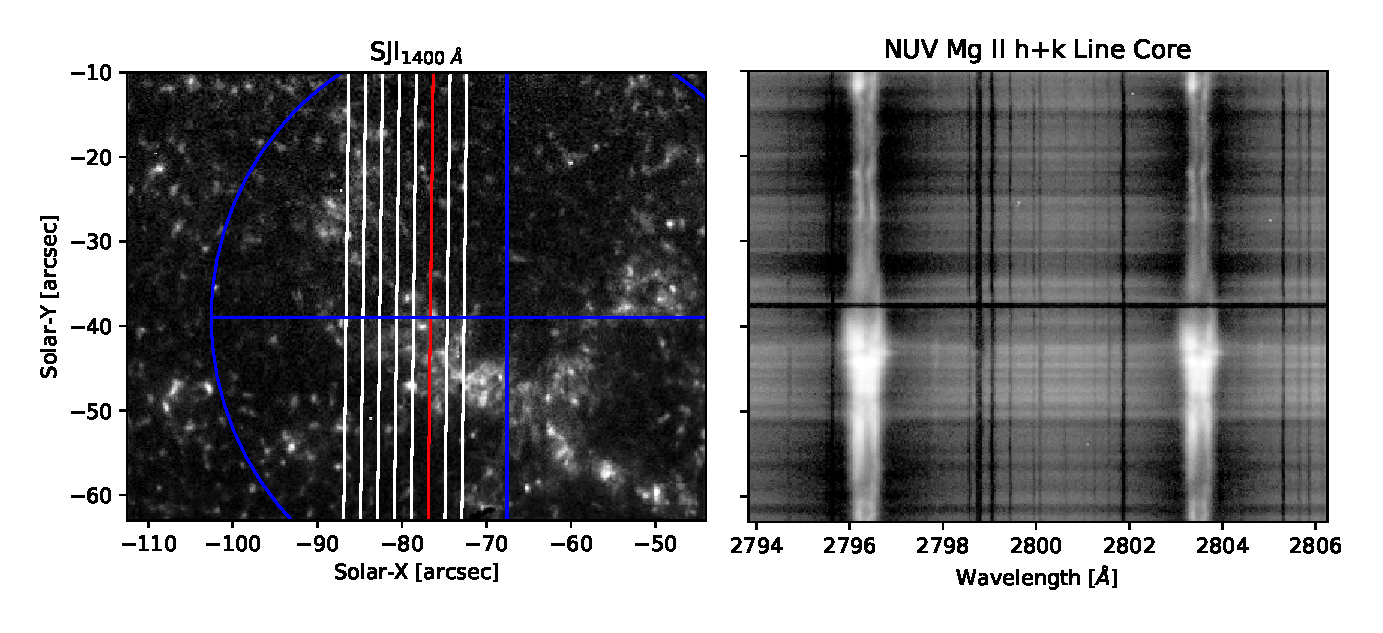
\includegraphics[width=7in]{./figures/IRIS_example.eps}
    \caption{An example of the IRIS Level 2 SJI and NUV spectrograph data near the time 15:47 UT.  The slit-jaw image is a composite of 4 images taken from 15:46:57.57 to 15:47:30.35 on 2017-03-21 to show the full field of view during the raster.  The slit positions for the 8-step coarse raster are shown over plotted on the SJI image in white.  The red slit indicates the position at which the NUV spectrum on the right was taken at 15:47:25.03.  The blue circle and crosshair shows the co-rotating ALMA field of view.}
    \label{fig:IRIS}
\end{figure*}

\subsection{{\it Hinode} SOT}
{\it Hinode} SOT Spectropolarimeter (SP) data was primarily taken from 14:00 UT to 18:46 UT with using 60 $\times$ 60 arcsec$^2$ fast maps with 0.3 arcsec spatial resolution with a $\sim$ 30 minute cadence. Additionally, the region of interest was observed sporadically over the 50 hours leading up to the coordinated observations, with FOVs of approximately $150\times160\unit{arcsec}^2$.  %The data was calibrated to level 2  using the BLAH method, and further reduced using Sarah's awesome skills. In total, this provided 7 maps of the region over the 50 hours leading up to the observation, and 10 maps of the region during the 4 hours of coordination.
The SP instrument performance is described in \citet{2013Litesetal}.

The SP Level 2 data, reduced and inverted with the Milne-Eddington gRid Linear Inversion Network (MERLIN) code to produce maps of physical atmospheric parameters, including the vector magnetic field, were obtained from the Community Spectropolarimetric Analysis Center (CSAC, DOI:10.5065/D6JH3J8D).  See \citet{2013Lites&Ichimoto} for a description of the data reduction routines.

\subsection{{\it Hinode} EIS}
EIS conducted observations for the coordinated campaign from 14:00 UT to 21:21 on 2017-03-21. This instrument provides a wide range of diagnostics as described in \citet{2007Young}. Context slot rasters approximately three minutes in duration were taken at the beginning and end of the observation.  In between the slot rasters, EIS took sit-and-stare observations with 34 sec cadence. The sit-and-stare observations were interrupted by a 10 minute disk center synoptic observation at 19:40 UT.

The EIS slot rasters covered a large region approximately $470\arcsec\times485\arcsec$ in 15 overlapping steps with spatial sampling of 1\arcsec\ per spatial pixel.  The sit-and-stare observations consisted of a 20\,s exposures with the 2\arcsec\ wide slit. Again, the spatial sampling along the slit was 1\arcsec\ per pixel. The detector readout for the spectra included all of the available wavelength ranges, but was limited to 256\arcsec\ along the slit. \saj{Where did the EIS data come from?  Harry probably got it from JSOC, I used VSO} The EIS data was processed using the default settings for the \verb+eis_prep+ routine in SSWIDL \citep{1998FreelandHandy_SSW}.  Intensities for the \ion{Fe}{12} 195.119\,\AA\ and \ion{He}{2} 256.317\,\AA\ lines were computed using multi-Gaussian fits \saj{reference or ssw routine name?}.

\begin{figure}
    \centering
    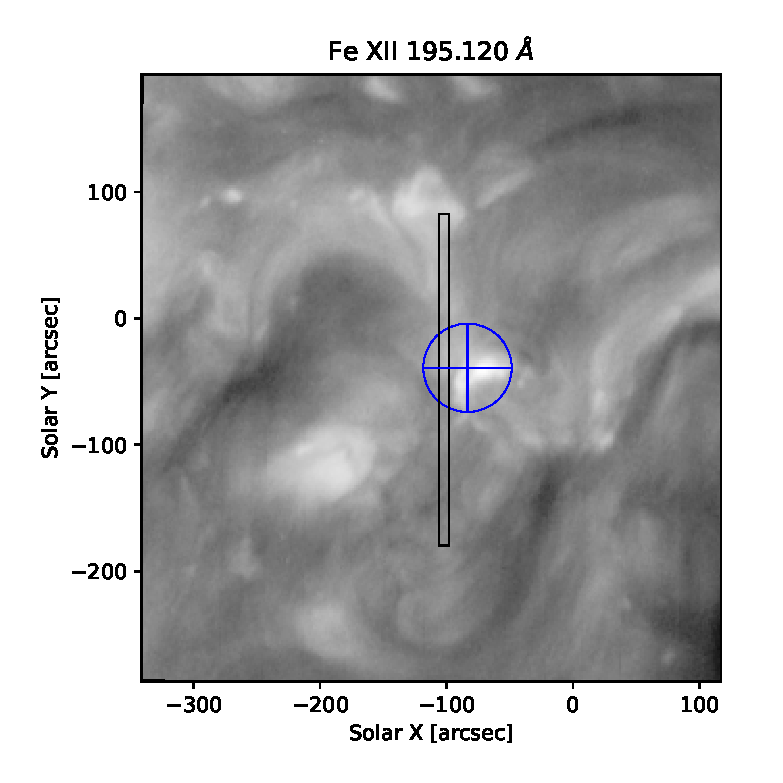
\includegraphics[width=3.5in]{figures/EIS_example.eps}
    \caption{A reconstructed slot raster image from the EIS \ion{Fe}{12} 195 \AA\ channel. The slot raster started at 14:00 UT.  The blue circle and crosshair show the ALMA co-rotating field of view.  The black rectangle shows the extent of the region covered by the EIS slit during the sit and stare observations.}
    \label{fig:EIS}
\end{figure}

\subsection{{\it Hinode} XRT}
XRT observed the active area from 12:33:12.311 -  18:59:27.511 UT with the Al\_poly filter, allowing plasma observations above $\sim$3 MK. The Al\_poly filter is one of the thinnest filters on XRT which has not been prohibitively impaired by contamination \citep[][]{2011NarukageEA_XRT3}, though some features of the contamination are still apparent. While the intended cadence was 4s, automatic exposure control increased the exposure time, which slowed the cadence to 16s per image. This large data series was prepped \citep[][]{2014KobelskiEA_xrtprep} and the methods of \citet{2015YoshimuraMcKenzie_XRTcoalign} were used to estimate offsets for co-alignment to the data to other instruments. Cross-correlation techniques \citep[such as {\tt tr\_get\_disp.pro} in SolarSoft;][]{1998FreelandHandy_SSW} were utilized to further remove instrumental jitter and to self-align the XRT data with itself.





\section{Co-alignment} \label{sec:coalign}
\begin{figure}[b]
    \centering
    \includegraphics[trim=200 100 100 100, clip, width=0.5\linewidth, angle=270]{figures/co-alignment.eps}
    \caption{Graphical representation of the coalignment process. SDO was utilized as the central coalignment reference, with other instruments co-aligned to it as possible. }\label{fig:coalign}
\end{figure}

Co-aligning the various instruments was a challenge.  
\figref{fig:coalign} graphically depicts how each data series was coaligned.
Our general approach was to use the broad wavelength and height coverage of the various HMI and AIA channels as a ``ground-truth'' mapping between solar coordinates and morphological features seen within each data series.
The 2012 Venus transit allowed subarcsecond alignment of all the AIA and HMI channels\footnote{See the SDO Data Analysis Guide at \url{https://www.lmsal.com/sdodocs/doc/dcur/SDOD0060.zip/zip/entry/}, \S{}7.1 in the Sept 14, 2020 version of the document.}, which has since been maintained using Mercury transit observations, making SDO an excellent resource for this task.  
Alignment was then verified by checking against data series that had not been explicitly aligned with each other.
For example, the IBIS broadband images were aligned to HMI continuum data and then that alignment was verified by checking the correspondence of enhanced emission in the \halpha{} line wings to the HMI magnetograms, SOT magnetograms, and UV emission in the 1600 and 1700\AA{} AIA channels. 

Each data series has different temporal and spatial samplings and physical extent so no attempt was made to resample images from each instrument to a common temporoal/spatial grid.  
Instead, the reduced and co-aligned data series make use of the World Coordinate System (WCS) variant for solar physics defined in \citet{2006Thompson} and included in the FITS headers.  
All data in this work uses helioprojective-cartesian coordinates, which can be transformed to any other coordinate system using standard routines in \fnc{SSW}, \fnc{astropy}, or \fnc{sunpy}.\par

\subsection{DST/FIRS}
FIRS data was co-aligned in two steps. First the FIRS slit-jaw images were co-aligned to HMI continuum intensity images from the 45s series, then the solar coordinates of the slit were mapped onto the spectrograph data.

During the reduction of the FIRS slit-jaw images, the FIRS slit and hairlines crossing the slit were fit in each image before application of the flat field.  The pixel coordinates of the slit/hairline pairs were saved for use during the co-alignment step.  The dark hairlines also appear in the FIRS spectrograph images.  During the reduction of the spectrograph data, the positions of these were also determined and saved for later use.

The reduced FIRS slit-jaw images were co-aligned to SDO/HMI intensity images from the 45 second series.  The approximate center coordinates of the FIRS slit-jaw were taken from the image headers which contain the telescope pointing near the time of the observation.  The spatial dispersion was estimated based on observations of the grid target.  The nearest HMI image in time was taken, and the coordinates were rotated to the time of the FIRS slit-jaw observation.  Using interpolation based on the estimated slit-jaw coordinates, a subfield was extracted from the HMI image.  X and Y shifts between the HMI sub-field and the slit-jaw image were determined using the SSW routine \verb+tr_get_disp+.  The spatial dispersion and rotation of the first image was adjusted by hand to achieve a good match, then the co-alignment of the entire image sequence was done using the same scale and rotation parameters.  The resulting coordinate mapping was used to transform the measured slit and hairline crossings into solar coordinates.  The FIRS slit-jaw images were written to FITS files with their updated coordinate information using the WCS standard.

To get the FIRS spectrograph data into the solar coordinate frame, the coordinates of the slit/hairline crossings for the slit-jaw data series were interpolated at the time of FIRS spectrograph observation.  The slit/hairline solar coordinates were then used to determine the spatial dispersion along the slit, the solar X and Y coordinates at the center of the slit, and the rotation of the slit with respect to solar north assuming a linear mapping.  Each set of polarized spectra was then written to a FITS file with the spatial and spectral coordinates in the WCS standard.  The Stokes I spectrum was written in the main extension, and the Stokes Q, U, and V states were written to subsequent extensions with abbreviated headers.

\begin{figure*}
    \centering
    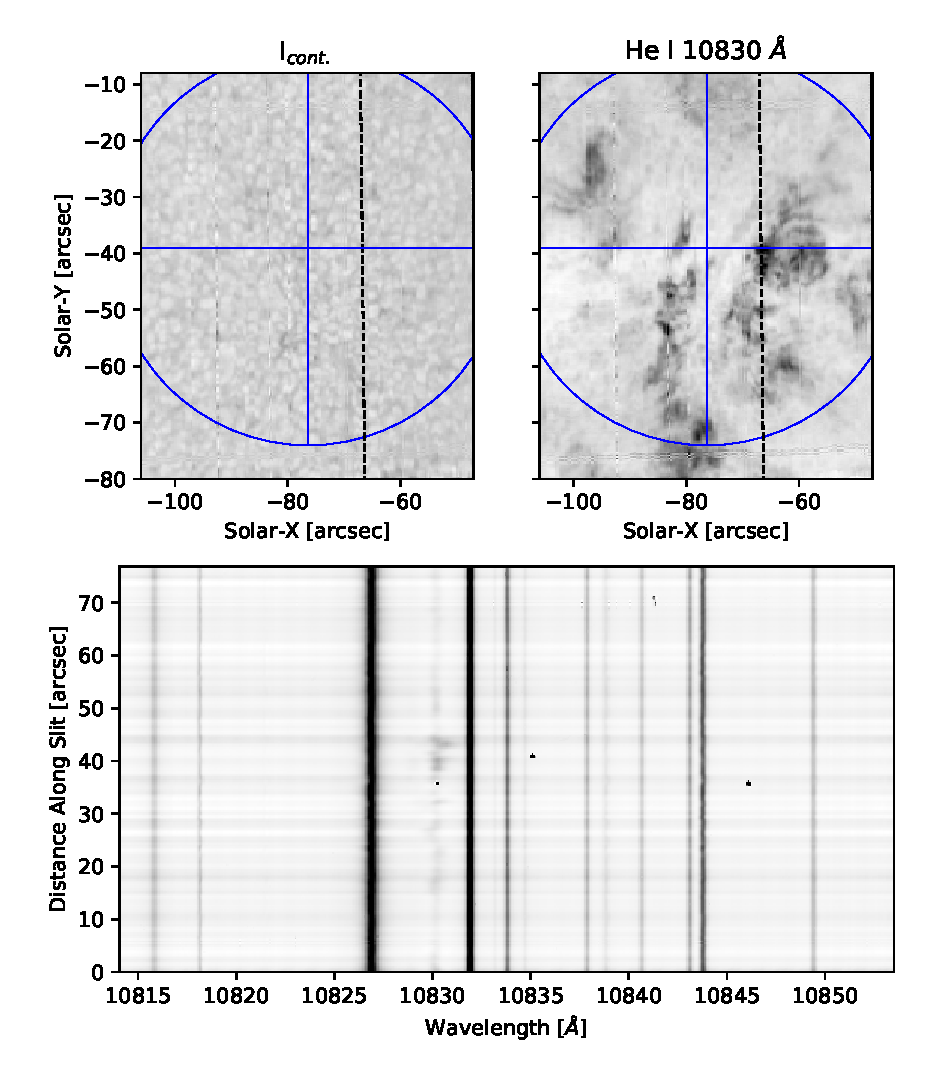
\includegraphics[width=5in]{./figures/FIRS_example.eps}
    \caption{co-aligned FIRS spectograph data from the beginning of the coordination taken between 14:46:48 and 15:00:55 UT on 2017-03-21.  The top two panels show the reconstructed maps of continuum and He I 10830 line intensity (left and right respectively).  The bottom panel shows the full Stokes I spectrum obtained with FIRS at 14:53:53 UT at the position indicated by the dashed line in each of the maps.  The blue circle and crosshair shows the co-rotating ALMA field of view.}
    \label{fig:FIRS}
\end{figure*}

\subsection{Hinode SOT}
%The Hinode SOT/SP parameter maps were resampled to a uniform coordinate grid, then aligned with HMI.

For each Level 2 raster scan of SOT/SP, the solar coordinates of the slit at each raster position were differentially rotated from the observed time to a common time at the center of the scan (using the SSW routine \verb+drot_xy+).  The parameter maps were then resampled to a uniform coordinate grid.  HMI intensity observations closest in time to the center of the SOT/SP scan were selected and interpolated onto the same coordinate grid and the relative shift between HMI and the SOT/SP continuum intensity map was determined (using \verb+tr_get_disp+).  SOT/SP coordinates were updated with the corresponding shift.  An ad-hoc rotation angle of CROTA2=-0.6 deg and x-y pixel scale of 0.315 arcsec/pixel were determined with respect to HMI and applied simultaneously with the coordinate shift.  The resampled and co-aligned SOT/SP parameter maps were written to WCS-compliant FITS files where the main extension contains continuum intensity, and the inverted parameters are contained in additional FITS image extensions.  Figure \ref{fig:SOTSP} shows an example of the continuum intensity and LOS magnetic field for the last large raster taken before the coordination with ALMA commenced.

\begin{figure*}
    \begin{center}
        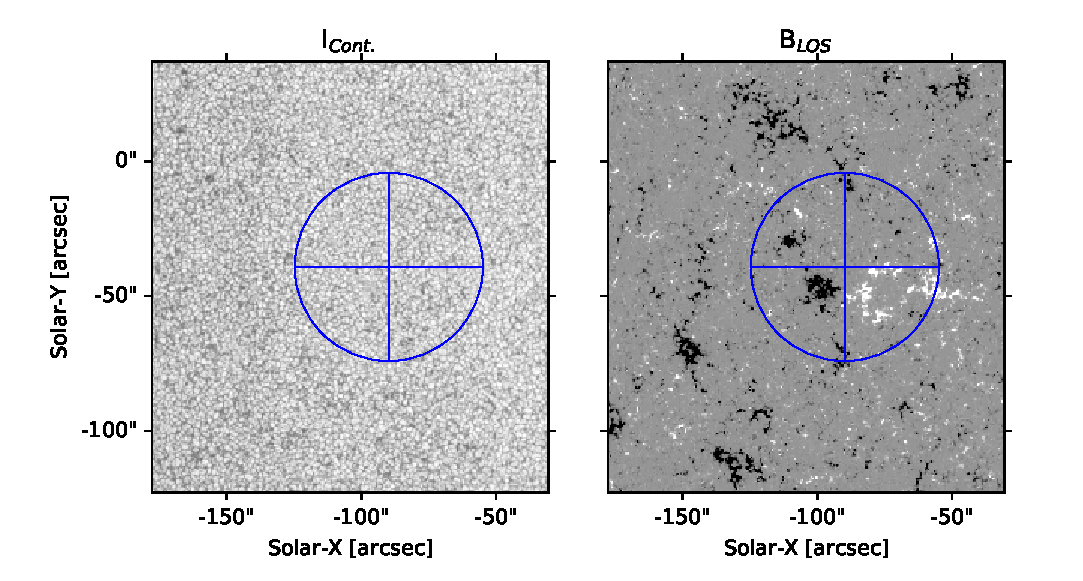
\includegraphics[width=7in]{./figures/SOTSP_example.eps}
    \end{center}
    \caption{The co-aligned continuum intensity and line of sight magnetic field from the co-aligned Level 2 SOT/SP data based on inversion of the 630.2 nm Fe I lines.  The raster scan was run from 13:16:01 to 13:48:21 UT on 2017-03-21, and was the last large raster taken before the coordinated sequence began.  The blue circle and crosshair shows the co-rotating ALMA field of view.}
    \label{fig:SOTSP}
\end{figure*}

\subsection{Hinode EIS}
The EIS slit data were co-aligned to 12\,s, $202\arcsec\times456\arcsec$ 193\,\AA\ AIA cutouts obtained from JSOC. For each EIS exposure we convolved the full CCD spectrum with the AIA effective area for the 193\,\AA\ channel. We also resampled the AIA images to better match the cadence and plate scale of the EIS data. We then cross correlated the EIS intensities along the slit with the the intensities in the resampled AIA image taken closest in time to the EIS exposure. We computed correlations over a range of positions close to the commanded pointing and recorded the position with the highest correlation. An example of co-aligned EIS and AIA intensities is shown in Figure \figref{fig:eis_aia}.

\begin{figure}
    \centering
    \includegraphics[width=0.85\linewidth]{./figures/eis_aia_108.pdf}
    \caption{Co-aligned EIS and AIA data. The left panel shows an AIA 193\,\AA\ image with the position of the EIS slit indicated by the black line. The AIA image was taken at 14:21:16:840, and the EIS image from 14:21:28:000. The center panel shows the EIS and AIA intensities along the slit. Note that the EIS intensities here are computed by convolving the spectrum with the AIA effective area. Intensities derived from Gaussian fits to the line profile were also computed. The right panel shows the EIS exposure in the vicinity of the \ion{Fe}{12} 195.119\,\AA\ line. }
    \label{fig:eis_aia}
\end{figure}

The EIS slot rasters at the beginning and end of the observations were also co-aligned to AIA 193 \AA\ images, but using a slightly different technique.  The EIS 195 \AA\ window was extracted for each slot position in the raster and the nearest AIA 193 \AA\ image in time was taken.  The EIS metadata values for rotation and spatial sampling of the EIS slot were adjusted, to $1^\circ$ and $1.00 \times 0.99$ arcsec respectively, for all slot data, and the center field position of each slot pointing was determined by eye to achieve a good match.  This rough pointing information was used to generate 2D helioprojective Cartesian coordinate arrays for the x and y coordinates of the image.  The AIA data was interpolated to the EIS coordinates, then the SSW routine \verb+tr_get_disp+ was used to determine the residual shift between the EIS and AIA images in an automated way.  These pixel shifts were then used to update the EIS coordinate arrays.

FITS files containing the EIS slot raster and spectrograph sit-and-stare co-aligned coordinates arrays are available with the data release accompanying this publication.  These co-aligned coordinates are only valid for the EIS 195 \AA\ wavelength because EIS has a systematic vertical shift with wavelength due to a small tilt of the grating \citep[e.g.][]{young09}.  Coordinate shifts relative to this wavelength should be applied based on the \verb+eis_ccd_offset+ routine in SSW.  Interested users are encouraged to obtain the original EIS data from JSOC or other sources and prep it with the latest routines for further for analysis.


\subsection{DST/IBIS}
The IBIS broad band images were aligned to HMI continuum images in order to determine the final IBIS coordinates.
All co-alignment steps used the \code{chi2\_shift} cross correlation routine and then were independently verified using the \code{phase\_cross\_correlation} routine from the \code{skimage.registration} Python package.
The co-alignment process found a $1.08^\circ$ rotation of the IBIS data to align the pixel array with the solar North-South axis, while the coordinates of the center IBIS pixel were determined to be $(-76.041, -52.032)$ at time 2017-03-21 14:47:05.164.
The center-pixel coordinates for all other times were then calculated from that $(x,y,t)$ triplet using the \code{solar\_rotate\_coordinate} routine from SunPy 2.0.3.
The final offsets from the IBIS self-alignment described in \secref{sec:ibisselfalign} and the rotation to align pixel axes with solar X-Y axes were simultaneously applied to both the broad band and narrow band data using the \code{affine\_transform} interpolation routine from Sunpy. 

Each IBIS FITS file contains data from a single exposure time, e.g., a single broad band and narrow band image pair.
The final coordinates were saved in the WCS compliant CRVAL1 and CRVAL2 fields of the FITS header for each IBIS data file, which apply to both the broad band and narrow band images, as part of the primary FITS header.
The broad band and narrow band data are saved in the first and second Image FITS extensions, respectively, along with additional header fields pertinent to each.
Because of the limited FOV, disk-center location, and short duration $(\sim 2\unit{hr})$ of these data, we did not consider image distortion due to the curved surface of the Sun, as such corrections would enter at sub-pixel scales.\par

\figref{fig:IBISgrid} shows representative IBIS data, including a broad band image of the solar granulation pattern and a subset of the wavelengths from the narrow band data.  The blue circle and cross shows the ALMA FOV at this time.

\begin{figure*}
    \centering
    \includegraphics[width=7in]{./figures/IBIS_ALMAcirc_grid}
    \caption{Co-aligned IBIS data for a partial scan through the \halpha{} line.  The scan began at 15:47:11.133UT and and lasted until 15:47:15.123, with approximately 0.165s between each narrow band image. The broad band data is in the upper left while remaining panels show a subset of the narrow band images.  The blue circle and crosshair shows the ALMA field of view at 15:47:13 UT.}
    \label{fig:IBISgrid}
\end{figure*}

\subsection{ALMA}\label{sec:almaalign}
As explained by \citet{2019Molnar}, variations in the Band-3 ALMA brightness temperature track variations in \halpha{} linewidth.
We therefore co-aligned the ALMA data to the IBIS-\halpha{} linewidths calculated using the method described in Section \secref{sec:linewidth}.
The ALMA data were shifted and rotated to center the beam at the center of the pixel array and align solar north-south axis aligned with pixel columns.  
The FOV center coordinates were then varied such that levelsets of the cotemporal ALMA and \halpha{} data aligned at beginning of the ALMA data series at time 2017-03-21 15:42:13.  
As with the IBIS data, the WCS compliant coordinate values `CRVAL1' and `CRVAL2' at all other times were calculated by rotating the co-aligned center pixel coordinates from the initial time using the \code{solar\_rotate\_coordinate()} routine from \code{Sunpy}.

\section{Analysis}\label{sec:analysis}
\subsection{Target Overview}
To get a baseline qualitative understanding of how the active area evolved leading up to our primary observations we applied the segmentation and feature tracking algorithms described in \citet{2012Tarr} to the $\approx330\times250\arcsec{}$ cutout of HMI data between 2017-03-19 00:00 and 2017-03-21 23:46UT.  
This analysis revealed fairly standard network behavior.
Throughout the entire FOV, magnetic concentrations cyclically coalesce and fragment.
On short timescales (several hours) the motion of flux concentrations appears coherent, but on longer time scales ($\sim1$ day) movement appears random.   

However, the observed motions are not completely random.
Our observations are centered on the bipolar grouping (positive magnetic fields to the West, negative to the East) shown in Figure \ref{fig:SOTSP} right.
Despite the continual fragmentation and coalescence, the bipole is present for the duration of the HMI data and is associated with persistent, short, bright coronal loops in the EUV and X-Ray data.
As described below, it is likely that the bipole emerged as a cohesive unit that is well into the decay phase, but it may simply be a long-lasting random bipolar concentration. 
For ease of language we will refer to it as ``the bipole.''

Considered from a global perspective, the positive polarity is parasitic within a roughly circular medium-scale ($\sim250\arcsec{}$ diameter) negative polarity region. 
The medium scale negative polarity region is itself surrounded by a larger scale, predominantly positive polarity region that extends across both sides of the solar equator.
This magnetic configuration makes the bipole topologically isolated from larger scale features: magnetic domains are layered somewhat like shells in an onion and we are interested in the dynamics of the inner layers.
This larger-scale configuration will inform MHD simulations to be presented in future work.

The pattern of a medium-scale dominant negative polarity surrounded by a larger scale positive polarity persisted for several solar rotations prior to our observations.
The bipole we are looking at is likely the decaying remains of AR 12639 which emerged around 2017-02-24 at $\approx$(10S, 30W).

Returning to the local scale of the bipole, overall during our observations it appears to be decaying, both by apparent direct cancellation between the two polarities and by fragmentation and separation of each polarity individually.
The general decay of the bipole is complicated by two other factors: (1) nearby small-scale emergence, for example, around $(-475,-50)\arcsec{}$ at time 2017-03-19 13:45UT, acts to replenish the decaying flux of each polarity, and (2) surrounding network concentrations that do not seem associated with emergence also random-walk into the bipolar region and replenish lost flux.

Finally, we note that immediately preceding our coordinated observations the parasitic positive polarity region of the bipole began an extended cycle of combined fragmentation and cancellation with the negative polarity of the bipole.
All of the processes describe above at the photospheric level likely drive both wave activity and continual reconnection higher in the atmosphere, resulting in the transient brightenings we describe below.

\subsection{IBIS Linewidths}
\label{sec:linewidth}
We characterized the spectral profile of \halpha{} at every spatial and temporal point of the IBIS data series.
Figure \ref{fig:linefitexample} shows a typical example of the spectral data (green crosses), including the Telluric oxygen line $\approx1.4\AA{}$ redward of the \halpha{} line center, pulled from a single pixel.
Fitting the spectral line serves dual purposes.
First, as stated above in \secref{sec:almaalign} and reported on by \citet{2019Molnar}, the \halpha{} linewidth is extremely useful for aligning the ALMA Band 3 data; we discuss this at length in the following subsections.
Second, the fitting produces several interesting plasma diagnostics of its own, including Doppler shifts and opacity fluctuations, which will be discussed in later publications.

Our spectral characterization followed the method of \citet{2009Cauzzi}.
First, we created a smooth model, $\hfit[\lambda]$ of the normalized spectra\footnote{Spectra at each spatial pixel at a given time were normalized to the intensity of the first measured wavelength position averaged over the central $600\times600$ pixels.  That wavelength is $6560.832$\AA{}, or $-1.9944$\AA{} relative to the center of the prefilter bandpass.} using the \scipy{} \fnc{interpolate} package, based on FITPACK.  
Second, we determine the location of the line center by fitting a 3-parameter Gaussian absorption profile to the central 11 points in the line core, spanning -0.7505 to 0.5687 \AA{} from the center of the IBIS prefilter:
\begin{equation}
    G[\lambda; b, \linecenter, a] = b- \sqrt{\frac{\log2}{\pi a^2}}\exp\Bigl(-\frac{(\lambda - \linecenter)^2}{a^2\log2}\Bigr)
\end{equation}
where $b$ is the continuum level, $\linecenter$ is the line center, and $a$ is the half-width-at-half-max value.  
We only use the line center value $\lambda_0$ of this fit because the fit to the line center is fairly good even though the \halpha{} line profile is poorly represented by a Gaussian.  \par

We combine the fitted line center and the spline model to define the remaining characteristics of the line.  
The value of the spline model at line center defines the minimum line intensity, $\imin{}=\hfit[\linecenter{}]$.  
Next, the line intensity at half the line depth is defined as the halfway point between the minimum intensity and average of the intensities at $\pm0.75$\AA{} from \linecenter{}: 
\begin{equation}
    \ihalf = \frac{1}{2}\Bigl(\frac{\hfit[\linecenter-0.75\text{\AA{}}]+\hfit[\linecenter+0.75\text{\AA{}}]}{2}+\imin \Bigr).
\end{equation}
Finally, the line width \linew{} is defined to be the difference between roots of the equation \mbox{$\hfit[\lambda]-\ihalf = 0$}, that is, the width of the line at intensity \ihalf.
\figref{fig:linefitexample} shows an example of the fitting method applied to a single profile.\par

\begin{figure}
    \centering
    \includegraphics[width=\linewidth]{figures/line-fit-example-figure.pdf}
    \caption{An example of the line fitting method, applied to the spectra at pixel $ix,iy=400,550$ at time 14:47:07.  The blue line with '+' symbols show the normalized spectra.  The green dashed line shows the spline interpolation to the data.  The orange line shows the gaussian fit to the spline model between $\approx-0.894$\AA{} and $0.8369$\AA{}.  \imin{} is marked by a red $\times$, the line intensities at $\linecenter\pm0.75$\AA{} by the green and purple dots, their average by the multi-color dot, the width--defining intensity level by the red stars, and the resulting line width by the dashed red line.}
    \label{fig:linefitexample}
\end{figure}

\subsection{Comparison of \halpha{} linewidth to ALMA brightness temperature}

\begin{figure*}
    \centering
    \includegraphics[width=\linewidth]{figures/IBIS_wdth_ALMA_tb_0100.png}
    \caption{\halpha{} line-core widths from IBIS (left) and the ALMA band 3 brightness temperature (right) at time 2017-03-21 15:45:34.  Contours of the ALMA brightness temperature are overlaid on both panels.  The white dashed circle shows the effective extent of ALMA's FOV.}
    \label{fig:almaibis}
\end{figure*}

The left panel of \figref{fig:almaibis} shows a spatial map of the \halpha{} linewidth at 15:45UT and the right panel shows the ALMA brightness temperature map from the same time.
The dashed circles in both panels show the approximate ALMA reconstruction FOV of $\sim60\arcsec{}$.
The contours in both panels are of the ALMA brightness temperature and clearly show the good correspondence between the \halpha{} line width and the ALMA brightness temperature.
It is also clear that the correspondence extends somewhat outside of the ALMA effective FOV before fading into the background noise level; this is as expected.
We have therefore verified the correlation between \halpha{} line widths and ALMA Band-3 brightness temperature, as reported by \citet{2019Molnar}.
An animation of \figref{fig:almaibis} shows good correlation over the entire 60mins of cotemporal observation, but full temporal analysis is outside the scope of the present discussion.

\citet{2019Molnar} synthesized the radiative emission from a range of model atmospheres, representative of quiet-Sun to strong plage conditions, using the RH code \citep{2001Uitenbroek}.  
Those results suggest that the broadening of \halpha{} as the chromospheric temperature rises is primarily an opacity effect due to an enhanced number density of H atoms in the $n=2$ quantum state, as opposed to broadening by thermal effects.  
They explained this behavior, extensively referencing \citet{2012Leenaarts}, as follows.  The \halpha{} source function is nearly uniform throughout the chromosphere.  
This feature gives \halpha{} its characteristic flat bottom, with fairly uniform intensity in wavelength moving away from line center, until a wavelength is reached at which the source function becomes sensitive to the photosphere, giving rise the the steep line wings.  
As the formation height of the line core increases, the transition to photospheric-dominated emission occurs further in wavelength from the line center.  

Now consider how this behavior changes as one varies the temperature of an atmospheric model.  
Moving from cooler to hotter models, two important things happen simultaneously \citep[see][Fig.~5]{2019Molnar}: (1) the $\tau=1$ surfaces for the \halpha{} line core and the ALMA Band 3 emission begin to coincide; and (2) the contribution functions for each line become more spatially localized higher in the atmosphere.
Thus, in the hotter models, which produce the largest \halpha{} linewidths and highest ALMA Band 3 brightness temperatures, essentially all the \halpha{} absorption occurs in a thin range of heights at the interface between the chromosphere and transition region, and coincides with the ALMA Band 3 millimeter emission.  
However, the above \halpha{} formation behavior, and the resulting correspondence between \halpha{} and ALMA millimeter emission, eventually breaks down for the hottest models that are most similar to active-regions, when the \halpha{} source function is no longer flat.  
We do not expect this break down to occur for the region of enhanced network we have targeted in this data set, with the result that we find good correspondence between the \halpha{} line width and ALMA brightness temperature throughout our observations.

The main result of this analysis is that we have verified the correspondence found by \citet{2019Molnar}.
Further, we have done so for a region of only slight enhanced network, rather than for an area of strong, active region plage.
If the radiative modeling described above is correct then we would expect stronger correlation of temporal dynamics in the hotter-ALMA/broader-\halpha{} than in the cooler-ALMA/narrower-\halpha{} regions.
Details of that temporal analysis will be presented in a forthcoming paper.

\subsection{Transient brightening detections}

In this data series, over 30 individual brightenings were detected in just XRT using the techniques of \citet{2014KobelskiEA_XRTTBs}. Most of the detections were found within overlapping fields of view (spatially and temporally) with the other instruments. A few brightenings overlap with EIS and IRIS slits, but we have not yet interpreted these specific features. These brightenings will be discussed in future work, with analysis that will be able to better detect and connect the transient activity and to determine whether there is increased and co-located chromospheric activity before and/or after these events. For now, we focus on a single example dynamic event, which was readily observed in most of the imaging data.  

\subsection{Transient brightening at 16:10-16:30}
We find evidence of a transient event in multiple data channels that appears to show energy transfer between the chromosphere to the corona and back along two different paths, between 16:10 and 16:30UT.
\figref{fig:coordination2} shows nine of our data channels near the end of the event.

The event starts as a strong, elongated dimming the \halpha{} blue wing, see especially the $-0.089\unit{nm}$ channel.
The dimming progresses roughly from SE to NW along the filament channel between the polarities of the bipole.
The ALMA data show cospatial enhanced temperatures during this time. A subset of these images is shown in Figure~\ref{fig:subset}.
\begin{figure*}
    \centering
    \includegraphics[width=\linewidth]{figures/IBISsubset_img0106.png}
    \caption{Subimage of the brightening event.}
    \label{fig:subset}
\end{figure*}

Small scale sympathetic event.

After brightening in ALMA the dynamic event then becomes visible in the hotter and higher data channels, especially AIA 304\AA{} and 193\AA{}, followed by XRT. 
The closeness with which the AIA light curves track each other suggests an initial brightening in the lower temperature component of the 193\AA{} which is then followed by brightening due to plasma heating the hotter component \citep[see details of the two 193\AA{} components shown in Figure~11 of ]{2012Boerner}, and followed in turn by the brightening observed with XRT. 
This strongly suggest that we are observing a direct heating event of the loop. 
\begin{figure*}
    \centering
    \includegraphics[width=\linewidth]{figures/evt01_lc_bb.eps}
    \caption{Sub-regions  shown in Figure~\ref{fig:lightcurves}. The bounding boxes were chosen from the AIA 304\AA image, and made wide enough to cover any lingering instrumental drifts and variations between wavelengths. The reference time is chosen to highlight the coronal counterpart, so occurs after the peak ALMA brightening. The XRT image has been reverse scaled to improve visibility. The wishbone feature is the prominent region of interest for this example. The brightening follows much of the same shape in all upper chromospheric and coronal wavelengths.}
    \label{fig:wishbonezoom}
\end{figure*}
\begin{figure}
    \centering
    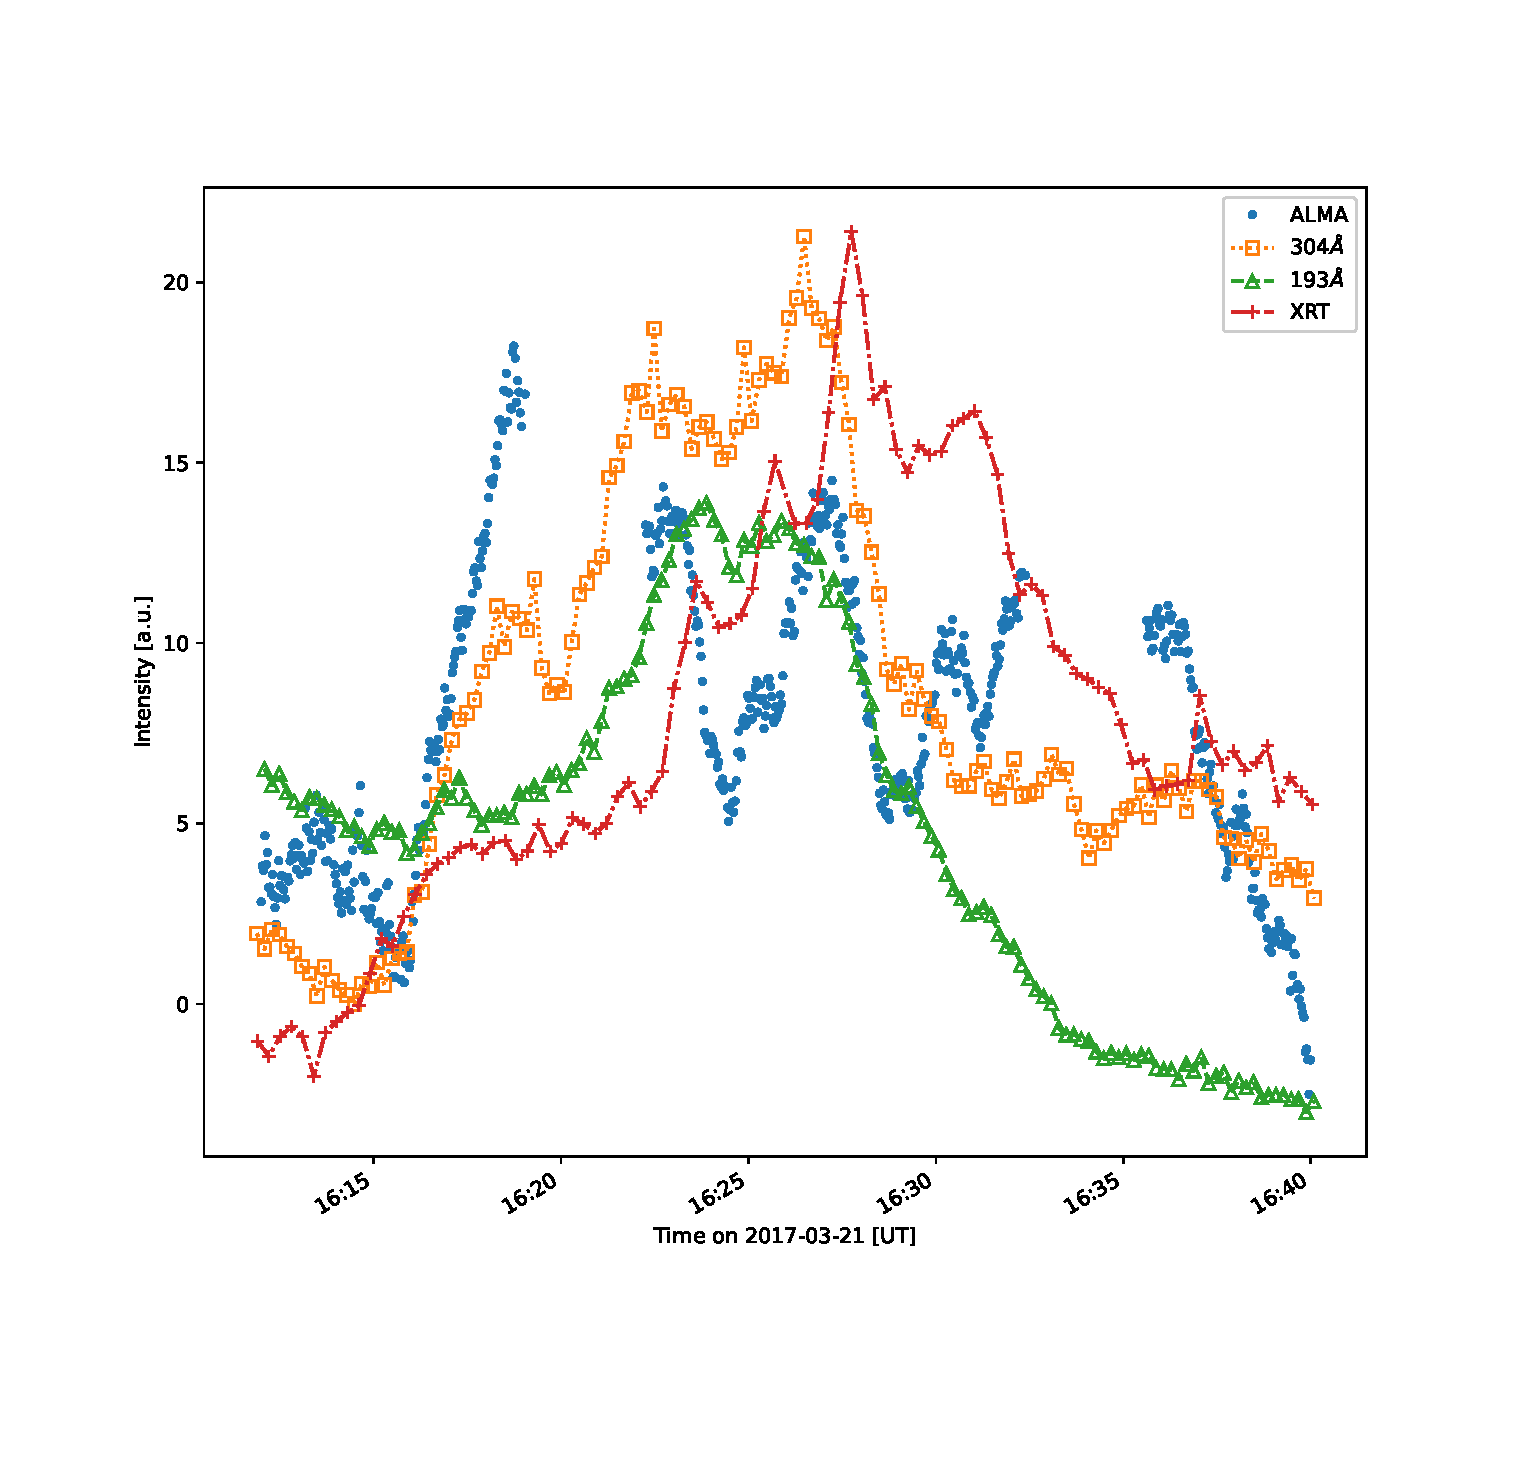
\includegraphics[width=\linewidth]{figures/evt01_lc_v2.eps}
    \caption{Light curves from sub-regions (will update figure~\ref{fig:subset} to outline) shown in Figure~\ref{fig:subset}. Here you can see that the brightening is initiated in the low chromosphere as shown with ALMA. The EUV data then brightens next, with the AIA 304\AA brightening slightly before the AIA 193\AA, though these brightenings follow much of the same shape.}
    \label{fig:lightcurves}
\end{figure}


Each the brightenings in the EUV and X-ray data follow the same progression from SE to NW along the filament channel, just as in the IBIS and ALMA data series.
The hotter channels then show a second loop brightening that partially overlaps the first but then extends southward from the negative concentration of the bipole towards a small flux concentration near the Southern edge of the ALMA field of view.
Finally we see a co-spatial and -temporal dimming in the \halpha{} blue wing and enhanced temperatures in ALMA at the Southern terminus of the secondary loop. 
The XRT data allow us to see the brightest thermal features in the region, which can be seen in the lower right panel of Figure~\ref{fig:coordination2} and in Figure~\ref{fig:wishbonezoom}. 
One of the most apparent features in the region during this time period, is the brightening along a new loop channel in the southern portion of the field of view.
This wishbone like loop feature is readily seen and outlined in the upper chromospheric and coronal channels and is shown Figure~\ref{fig:wishbonezoom}.
Lightcurves of the bounded region of the wishbone feature are shown in Figure~\ref{lightcurves}. 
The light curves clearly show the pre-brightening in the low chromosphere with ALMA, followed by the hotter channels.
Similar to the methods discussed in \citet{2014KobelskiEA_XRTTBs} and \citet{2014KobelskiMcKenzie_HiC}, we have searched for small, dynamic brightenings in the data. 





\section{Conclusions}\label{sec:conclusion}
We have presented an extensive coordinated data set that includes data series from multiple facilities and, in some cases, multiple instruments from each facility.
We describe the calibration and self-alignment of each data series and the coalignment of all data series within the data set.
The fully calibrated and aligned data are publicly available at \url{https://share.nso.edu/shared/dkist/ltarr/kolsch/}.
The coordination was keyed to our ALMA Cycle 4 observations which targeted a bipolar region of enhanced network for approximately one hour starting at 14:42 UT on 2017-03-21.
The target was situated close to disk center, approximately $(-70,-50\arcsec{})$ at the center of the ALMA data series. 
The other data series cover a variety of fields-of-view, start times, and durations.

We found that the spatial areas of broadest line width of the \halpha{} spectral line as observed by IBIS were cospatial to the hottest regions as measured by ALMA Band 3 $(\gtrsim 7500\unit{K})$.
This correspondence held for the entire duration of the ALMA observations.
This result extends the findings of \citet{2019Molnar}, who analyzed a single time frame of active region plage, to quiescent solar regions and extended time durations.
A future work will discuss the statistics of temporal dynamics between the two data series.

Preliminary analysis found multiple transient brightenings throughout the data set, some of which span multiple data series.
We highlight one particularly well observed example lasting approximately 20 minutes starting at 16:10 UT.
Lightcurves of the event show a clear transition from lower to higher temperature data series, starting in the chromospheric ALMA data ($\sim7000\unit{K}$) and progressing up to our hottest observed thermal series in \textsl{Hinode}/XRT ($\sim3\unit{MK}$).
Spatially, the event shows a propagation first along a filamentary feature above the central polarity inversion line of the bipole and then a secondary Y-shaped extension to another network concentration approximately $15\arcsec$ to the South. 
\ark{potentially also add SALSA info}.
What this data demonstrates is that these small scale events with large wavelength coverage are interesting, and cover some of the same dynamic features as seen in larger events. We hope the community is able to further utilize this small but robust data set.





\acknowledgments
%ALMA
This paper makes use of the following ALMA data: ADS/JAO.ALMA$\#$2016.1.00788.S. ALMA is a partnership of ESO (representing its member states), NSF (USA) and NINS (Japan), together with NRC (Canada), MOST and ASIAA (Taiwan), and KASI (Republic of Korea), in cooperation with the Republic of Chile. The Joint ALMA Observatory is operated by ESO, AUI/NRAO and NAOJ.

%DST
Data in this publication were obtained with the Dunn Solar Telescope of the National Solar Observatory, which is operated by the Association of Universities for Research in Astronomy, Inc., under cooperative agreement with the National Science Foundation.  

%IRIS
IRIS is a NASA small explorer mission developed and operated by LMSAL with mission operations executed at NASA Ames Research center and major contributions to downlink communications funded by ESA and the Norwegian Space Center.
The authors thank K.~Reardon for help calibrating the IBIS data.

%Hinode SOT/SP done in text
Hinode is a Japanese mission developed and launched by ISAS/JAXA, collaborating with NAOJ as a domestic partner, NASA and STFC (UK) as international partners. Scientific operation of the Hinode mission is conducted by the Hinode science team organized at ISAS/JAXA. This team mainly consists of scientists from institutes in the partner countries. Support for the post-launch operation is provided by JAXA and NAOJ(Japan), STFC (U.K.), NASA, ESA, and NSC (Norway).

This research has made use of NASA’s Astrophysics Data System.
%% To help institutions obtain information on the effectiveness of their 
%% telescopes the AAS Journals has created a group of keywords for telescope 
%% facilities.
%
%% Following the acknowledgments section, use the following syntax and the
%% \facility{} or \facilities{} macros to list the keywords of facilities used 
%% in the research for the paper.  Each keyword is check against the master 
%% list during copy editing.  Individual instruments can be provided in 
%% parentheses, after the keyword, but they are not verified.

\vspace{5mm}
\facilities{ALMA, Dunn(FIRS, IBIS), IRIS, SDO(AIA, HMI), Hinode(EIS, SOT, XRT)}

%% Similar to \facility{}, there is the optional \software command to allow 
%% authors a place to specify which programs were used during the creation of 
%% the manuscript. Authors should list each code and include either a
%% citation or url to the code inside ()s when available.

\software{\code{astropy} \citep{2013astropy,2018astropy}, \code{sunpy} \citep{2020sunpy}, \code{numpy} \citep{2020Harris}, \code{sswidl} \citep{1998FreelandHandy_SSW}}

%% Appendix material should be preceded with a single \appendix command.
%% There should be a \section command for each appendix. Mark appendix
%% subsections with the same markup you use in the main body of the paper.

%% Each Appendix (indicated with \section) will be lettered A, B, C, etc.
%% The equation counter will reset when it encounters the \appendix
%% command and will number appendix equations (A1), (A2), etc. The
%% Figure and Table counter will not reset.

\bibliographystyle{yahapj}
\bibliography{references}
%\comment{
%\begin{thebibliography}{}

%\bibitem[Astropy Collaboration et al.(2013)]{2013A&A...558A..33A} Astropy Collaboration, Robitaille, T.~P., Tollerud, E.~J., et al.\ 2013, \aap, 558, A33 

%\end{thebibliography}
%}
%% This command is needed to show the entire author+affilation list when
%% the collaboration and author truncation commands are used.  It has to
%% go at the end of the manuscript.
%\allauthors

%% Include this line if you are using the \added, \replaced, \deleted
%% commands to see a summary list of all changes at the end of the article.
%\listofchanges

\end{document}

% End of file `sample62.tex'.
